\documentclass[12pt,a4paper,handout]{beamer}

\usefonttheme{professionalfonts}
%\usepackage[ngerman]{babel}% deutsches Sprachpaket wird geladen
\usepackage[ngerman,english]{babel}% englisches Sprachpaket wird geladen
\usepackage{tabularx}
\usepackage{lmodern}% Für die Schrift
\usepackage[T1]{fontenc} % westeuropäische Codierung wird verlangt
\usepackage[utf8]{inputenc}% Umlaute werden erlaubt
\usetheme{Berlin}
%\usepackage{showkeys} % Labels anzeigen
\usepackage{amsmath} % Erweiterung für den Mathe-Satz
\usepackage{amssymb} % alle Zeichen aus msam und msmb werden dargestellt
\usepackage{framed}
\usepackage[german]{fancyref}
\usepackage{listings}
\usepackage{color}
\definecolor{mygreen}{RGB}{28,172,0} % Define colour
\definecolor{mylilas}{RGB}{170,55,241}
\usepackage{graphicx} % Graphiken und Bilder können eingebunden werden
\usepackage{multirow} % erlaubt in einer Spalte einer Tabelle die Felder in mehreren Zeilen zusammenzufassen
\usepackage{url} % Dient zur Auszeichnung von URLs; setzt die Adresse in Schreibmaschinenschrift.
\usepackage[center]{caption}  % Bildunterschrift wird zentriert
\usepackage{subfigure} % mehrere Bilder können in einer figure-Umgebung verwendet werden
\usepackage{longtable} % Diese Umgebung ist ähnlich definiert wie die tabular-Umgebung, erlaubt jedoch mehrseitige Tabellen.
\usepackage{amsthm} % erlaubt die Benutzung von eigenen Theoremen
\usepackage{hyperref} % Links und Verweise werden innerhalb von PDF Dokumenten erzeugt
\usepackage{wrapfig} % Das Paket ermöglicht es von Schrift umflossene Bilder und Tabellen einzufügen.
%\numberwithin{equation}{section} % Nummerierungen der Gleichungen, die durch equation erstellt werden, sind gebunden an die section
\usepackage{latexsym} % LaTeX-Symbole werden geladen
\usepackage{tikz} % Erlaubt es mit tikz zu zeichnen
\usepackage{tabularx} % Erlaubt Tabellen 
\usepackage{algorithm} % Erlaubt Pseudocode
\usepackage{algorithmic}
\usepackage{color} % Farbpaket wird geladen
\usepackage{stmaryrd} % St Mary Road Symbole werden geladen
\usepackage{csquotes}
\usepackage{bm}
\usepackage{todonotes}
\usepackage{lipsum}
\usepackage{multicol}
\usepackage{multimedia}

% Hier werden neue Theorems erstellt.
\theoremstyle{definition}
\newtheorem{auf}{Aufgabe}
\newtheorem{rem}[auf]{Remark}
\newtheorem{defn}[auf]{Definition}
\newtheorem{bsp}[auf]{Example}
\newtheorem{notation}[auf]{Notation}
\theoremstyle{plain}
\newtheorem{kor}[auf]{Corollary}
\newtheorem{sa}[auf]{Theorem}
\newtheorem{lem}[auf]{Lemma}
\newtheorem{alg}[auf]{Algorithm}
\DeclareMathOperator*{\esssup}{ess\,sup} % essentiellen Supremums
\DeclareMathOperator{\spn}{span} % Span
\DeclareMathOperator{\supp}{supp} % Träger
\DeclareMathOperator{\ddiv}{div} % divergenz
\newcommand{\abs}[1]{\left\vert #1\right\vert}
\newcommand{\dotp}[2]{\left\langle #1,#2\right\rangle}
\newcommand{\rr}{\mathbb{R}}
\newcommand{\g}{~\textgreater ~}
\newcommand{\ls}{~\textless ~}
\renewcommand{\algorithmicrequire}{\textbf{Input:}}
\renewcommand{\algorithmicensure}{\textbf{Output:}}
\newcommand{\cc}{\mathbb{C}}
\newcommand{\kk}{\mathbb{K}}
\newcommand{\nn}{\mathbb{N}}
\newcommand{\qq}{\mathbb{Q}}
\newcommand{\e}{\varepsilon\g 0~}
\newcommand{\fe}{\forall \e}
\newcommand{\so}{\sum_{k=0}^{n}}
\newcommand{\si}{\sum_{k=1}^{n}}
\newcommand{\soi}{\sum_{k=0}^{\infty}}
\newcommand{\sii}{\sum_{k=1}^{\infty}}
\newcommand{\de}{\mathrm{d}}
\newcommand{\norm}[1]{\left\lVert#1\right\rVert}
\newcommand{\lpnorm}[1]{\left(\int\abs{#1}^2\D\Omega \right)^{1/2}}
\newcommand{\bfu}{\bm{u}}
\newcommand{\bff}{\bm{f}}
\newcommand{\bfB}{\bm{B}}
\newcommand{\bfb}{\bm{b}}
\newcommand{\bfs}{\bm{s}}
\newcommand{\bfC}{\bm{C}}
\newcommand{\bfx}{\bm{x}}
\newcommand{\bfR}{\bm{R}}
\newcommand{\D}{\mathop{}\!\mathrm{d}}
\floatname{algorithm}{Algorithmus}
%\renewcommand{\thesubfigure}{the.g}
\addto{\captionsenglish}{\renewcommand{\bibname}{References}}
\lstset{language=Matlab,
    basicstyle={\scriptsize \ttfamily},
    breaklines=true,
    morekeywords={matlab2tikz},
    keywordstyle=\color{blue},
    morekeywords=[2]{1}, 
    keywordstyle=[2]{\color{black}},
    identifierstyle=\color{black},
    stringstyle=\color{mylilas},
    commentstyle=\color{mygreen},
    showstringspaces=false, %without this there will be a symbol in the places where there is a space
    numbers=left,
    numberstyle={\tiny \color{black}}, % size of the numbers
    numbersep=9pt, % this defines how far the numbers are from the text
    emph=[1]{for,end,break},
    emphstyle=[1]\color{red}, %some words to emphasise
}
\makeatletter
\renewcommand{\p@subfigure}{}
\renewcommand{\@thesubfigure}{\thesubfigure:\hskip\subfiglabelskip}
\makeatother
\begin{document}
    \title{Numerical Solution of Integro-Differential Equations}
    \author{Nils Dornbusch}
    \date{July 09, 2019}
    \maketitle
    \begin{frame}
    \tableofcontents[pausesections]
    \end{frame}
\section{Introduction}
\frame{
    \frametitle{Introduction}
    A Non-Newtonian fluid is a fluid that changes its viscosity under stress.
        There are many examples for them. These include
        \begin{itemize}[<+->]
        \item toothpaste
        \item liquid plastic
        \item granular flow
        \item and many more.
        \end{itemize}}
\begin{frame}
    \frametitle{Motivation}
    \begin{itemize}[<+->]
        \item Simulation of this particular fluid model does not exist 
        \item First step in trying to develop a stable numerical approach
        \item To develop a starting point for future projects
    \end{itemize}
\end{frame}
\section{Physics}
    \begin{frame}
        \frametitle{Physics}
        \begin{itemize}[<+->]
            \item  The physical model uses the well-known Navier Stokes equations
            \item The stress tensor is modeled using an integral model
        \end{itemize}
    \end{frame}

       \begin{frame}
        \frametitle{The incompressible Navier Stokes equations}
        \begin{align*}
        \frac{\partial \bfu}{\partial t}+(\bfu\cdot \nabla)\bfu &= \bff +\nabla\cdot\sigma +\mu_s\Delta\bfu-\nabla p,\\
        \ddiv(\bfu)&= 0,\label{eq:div0}\\
        \sigma(t,\hat\bfx)&= \int_{-\infty}^t-\partial_{t'}\bfB(t,t',\hat\bfx)G(t,t')\D t',\\
        \partial_t \bfB &=- (\bfu\cdot\nabla)\bfB+(\nabla \bfu)\bfB+\bfB(\nabla\bfu)^T.
        \end{align*}
        with e.g. $G(t,t')=\mu_p\cdot e^{-(t-t')/\lambda}$, $\bfu$ the velocity vector, $\bff$ a generic source term, $\sigma$ the stress tensor, $\mu_s, \mu_p$ the solvent and polymer viscosity respectively, $p$ the pressure, $\lambda$ the relaxation time and $\bfB$ the Finger tensor.
     \end{frame}
 \begin{frame}
     \frametitle{Boundary conditions}
     We choose suitable initial and boundary conditions for the velocity. For $\bfB$ we use
     \begin{align*}
         \bfB(t,t,\hat\bfx)& = \bm{1},\\
         \bfB(0,t',\hat\bfx) &=\bm{1},
     \end{align*}
     which means that we assume a stress free start of the simulation.
 \end{frame}
\section{Dimension reduction}
    \begin{frame}
        \frametitle{Assumptions for the dimension reduction}
        These are very complex equations. This work uses the following assumptions:
        \begin{itemize}[<+->]
            \item $\bfu= (0,0,u)^T$, $\bff=\bm{0}$, $\nabla p\equiv(0,0,\partial_3 p)$
            \item $\partial_3\bfB =\bm{0}$
         \end{itemize}
    \uncover<3->{This yields a 2D model for the cross sectional flow in a e.g. tube.}\\
    
    \only<4>{\begin{figure}
            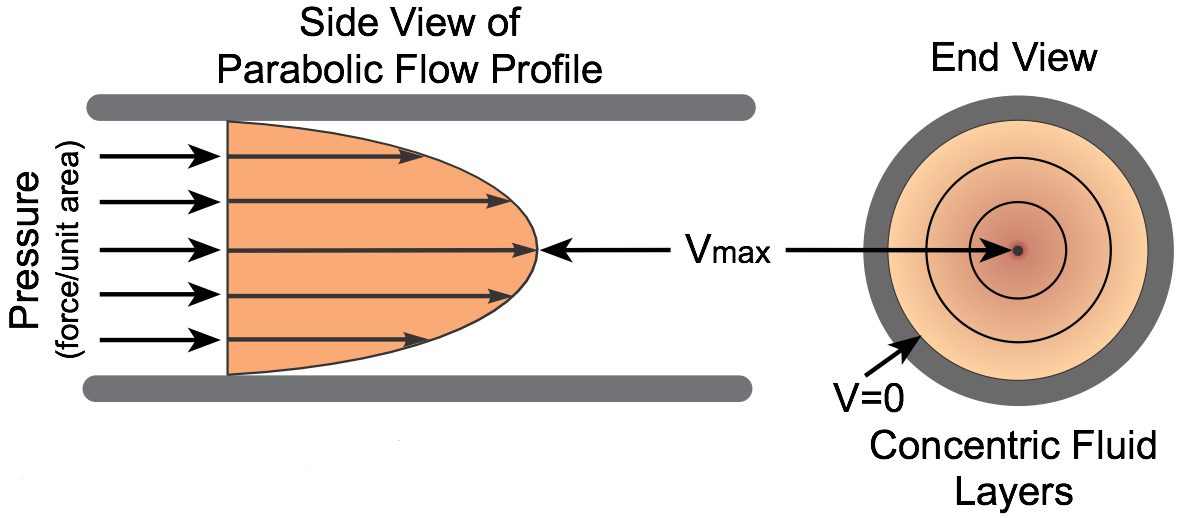
\includegraphics[width=0.5\textwidth]{h006-laminar-flow}
            \caption{Visualization of the assumptions (reference in the thesis)}
         \end{figure}}
    \end{frame}
\begin{frame}
    \frametitle{Dimension reduction}
    We observe
    \begin{itemize}[<+->]
        \item $0=\ddiv u = \partial_3 u$
        \item therefore $(\bfu\cdot\nabla)\bfu=(0,0,u\partial_3 u)= \bm{0}$
        \item $\Delta \bfu = (0,0,\Delta u) = (0,0,\Delta_{2D}u)$
    \end{itemize}
\end{frame}
\begin{frame}
    \frametitle{Dimension reduction}
    Recall $\partial_t \bfB =- (\bfu\cdot\nabla)\bfB+(\nabla \bfu)\bfB+\bfB(\nabla\bfu)^T$
    \begin{itemize}[<+->]
        \item we get $\partial_t \bfB_{i,j}=-u(\partial_3 \bfB_{i,j})$ for $(i,j)\in\{1,2\}^2$
        \item because $\partial_3 \bfB =\bm{0}$ we know that this block is constant in time
        \item according to initial condition we choose the identity for this block
        \item only last row/column of interest
        \item recall $\partial_3 \bfB_{3,3}=0$
        \item new variable $\bfb=\bfB_{3,j}$ for $j=1,2$
        \item and $\bfs(t,\hat\bfx) =\int_{-\infty}^t-\partial_{t'}\bfb(t,t',\hat\bfx)G(t,t')\D t'$.
    \end{itemize}  
\end{frame}
\begin{frame}
    \frametitle{Dimension reduction}
    To visualize the previous ideas:
    \begin{equation*}
    \bfB=\begin{pmatrix}
        1&0&\bfb_1\\
        0&1&\bfb_2\\
        \bfb_1&\bfb_2&*
    \end{pmatrix}
    \end{equation*}
\end{frame}
\begin{frame}
    \frametitle{Dimension reduction}
    Finger tensor equation in index notation
    \begin{equation*}
    \partial_t \bm{B}_{i,j}+\sum_{k=1}^3\bm{u}_k\partial_k \bm{B}_{i,j}-\sum_{k=1}^3\partial_k\bm{u}_i\bm{B}_{k,j}-\sum_{k=1}^3\bm{B}_{i,k}\partial_k\bm{u}_j=0
    \end{equation*}
    transforms to
    \begin{equation*}
    \partial_t \bfb_j -\sum_{k=1}^2\partial_ku\bm{B}_{k,j}=0.
    \end{equation*}
\end{frame}
\begin{frame}
    \frametitle{Dimension reduction}
    2D equations 
    \begin{align*}
    \partial_t u(t,\bfx) &= -\partial_3 p +\nabla\cdot \bfs+\mu_s\Delta u,\\
    \bfs(t,\bfx) &=\int_{-\infty}^t-\partial_{t'}\bfb(t,t',\bfx)G(t,t')\D t',\label{eq:s2D}\\
    \partial_t\bfb(t,t',\bfx)&=
    \begin{pmatrix}
    \partial_1 u(t,\bfx)\\\partial_2 u(t,\bfx)
    \end{pmatrix}=\nabla u.
    \end{align*}
\end{frame}
\section{Laplace transform}
\begin{frame}
    \frametitle{Laplace transform}
    We want to eliminate the integral. Our solution: 
    \begin{enumerate}[<+->]
        \item introduce $\tau= t-t'$ (age variable)
        \item put this into the equations
        \item perform the Laplace transform of $\bfb$ with respect to $\tau$
    \end{enumerate}
\end{frame}
\begin{frame}
    \frametitle{Laplace transform}
    The equation for the stress tensor with $\tau$ reads
    \begin{equation*}
        \bfs(t,\bfx)=\int_0^\infty\partial_\tau\bfb(t,t-\tau,\bfx)G(t,t-\tau)\D\tau.
    \end{equation*}
   Using the chain rule the governing equation for the Finger tensor transforms to  
   \begin{equation*}
   \partial_t \bfb +\partial_\tau\bfb=\nabla u
   \end{equation*}
\end{frame}
\begin{frame}
    \frametitle{Laplace transform}
    Transform $\bfb\mapsto L_b:=\int_0^\infty \bfb(x,t,t-\tau)e^{-s\tau}\D \tau$. This yields
    \begin{equation*}
    \partial_tL_{\bfb}(t,\bfx,s) + L_{\partial_\tau\bfb}(t,\bfx,s) = \frac{1}{s}\nabla u.
    \end{equation*}
    Second part of the sum:
        \begin{align*}
        L_{\partial_\tau\bfb}(t,\bfx,s) &= \int_0^\infty\partial_\tau\bfb(t,t-\tau,\bfx)e^{-s\tau}\D\tau\\ &=\lim_{r\to\infty}\bfb(t,t-r,\bfx)e^{-sr}-\bfb(t,t,\bfx)e^{-s\cdot 0}\\&+s\int_0^\infty\bfb(t,t-\tau,\bfx)e^{-s\tau}\D\tau.\\
        &= -\bfb(t,t,\bfx) +sL_{\bfb}(t,\bfx, s)\\
        &= sL_{\bfb}(t,\bfx,s).
        \end{align*}
\end{frame}
\begin{frame}
    \frametitle{Laplace transform}
    Using $C_s:=sL_b(t,\bfx,s)$ we obtain
    \begin{equation*}
         \partial_t\bfC_s(t,\bfx)+s\bfC_s(t,\bfx)=\nabla u
    \end{equation*}
    Until now no assumptions on the function type of $G$ were made.
    If we set $s:=\frac{1}{\lambda}$ and use $G(t,t-\tau)=\mu_pe^{-\tau/\lambda}$, it follows
    \begin{equation*}
        \bfs(t,\bfx)=\mu_pC_{1/\lambda}(t,\bfx)
    \end{equation*}
\end{frame}
\begin{frame}
    \frametitle{The transformed 2D equations}
    \begin{align*}
        \partial_t u(t,\bfx) &= -\partial_3 p +\nabla\cdot \bfs+\mu_s\Delta u,\\
        \label{eq:transfeq2}
        \bfs(t,\bfx)&=\mu_p\bfC_{1/\lambda},\\
        \partial_t\bfC_{1/\lambda}(t,\bfx) &= -\frac{1}{\lambda}\bfC_{1/\lambda}(t,\bfx)+\frac{1}{\lambda}\nabla u    \end{align*}
        This is a linear system of which the existence and uniqueness of the solution is proven in the thesis.
\end{frame}
\section{Numerics}
\begin{frame}
    \frametitle{The software}
    The software used is FEniCS. 
    \begin{itemize}[<+->]
        \item Framework for solving PDEs with finite element discretization (limited DG support available)
        \item have to plug in the weak form and maybe time loop
        \item MPI support, however not tested yet 
    \end{itemize}
    \begin{figure}
        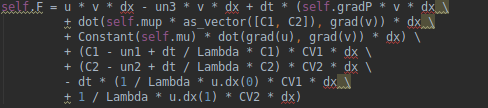
\includegraphics[width=0.5\textwidth]{FenicsCode}
        \caption{Weak formulation for the derived equations with timestepping}
    \end{figure}
\end{frame}
\begin{frame}
\frametitle{Simulation cases}
The following cases were simulated
\begin{itemize}[<+->]
    \item Circle mesh 
    \begin{itemize}[<+->]
        \item Startup flow with a fixed pressure 
        \item Flow with manufactured solution for convergence
    \end{itemize}
    \item square mesh (side length = 2)
    \begin{itemize}[<+->]
        \item cross section of an ideal rheometer
    \end{itemize}
\end{itemize}
\uncover<6>{Note: Units have been omitted but have to be chosen consistently. }
\end{frame}
\begin{frame}
    \frametitle{Numerical results}
    Two domains: circle and square
    \begin{figure}
        \caption{Meshes with }
        \subfigure[402987 cells]{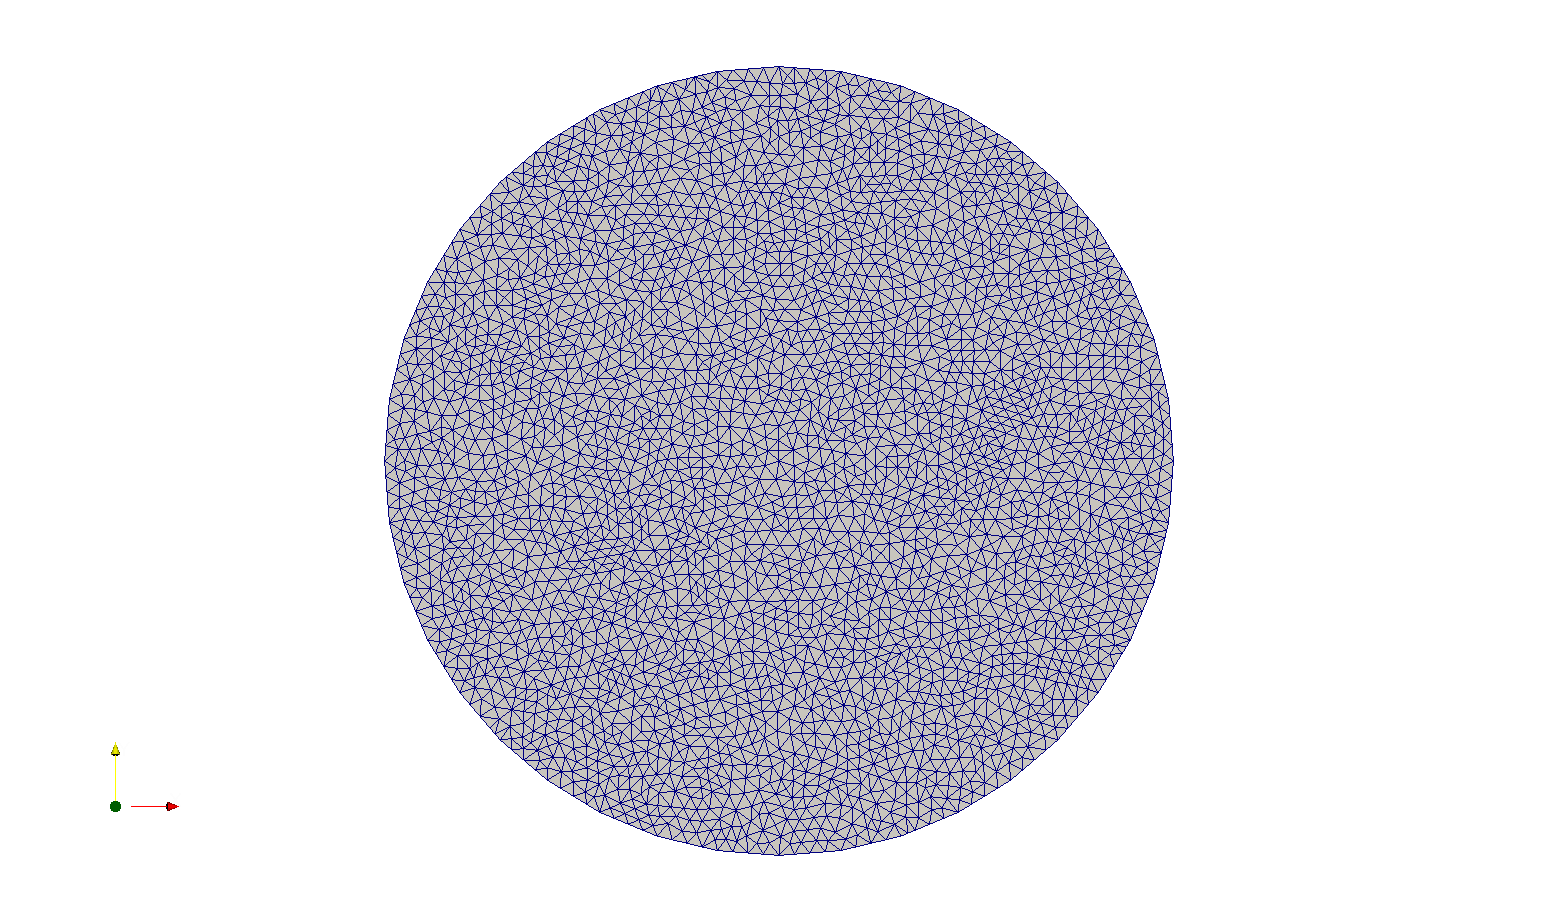
\includegraphics[width=0.4\textwidth]{MeshCircle}}
        \subfigure[4852 cells]{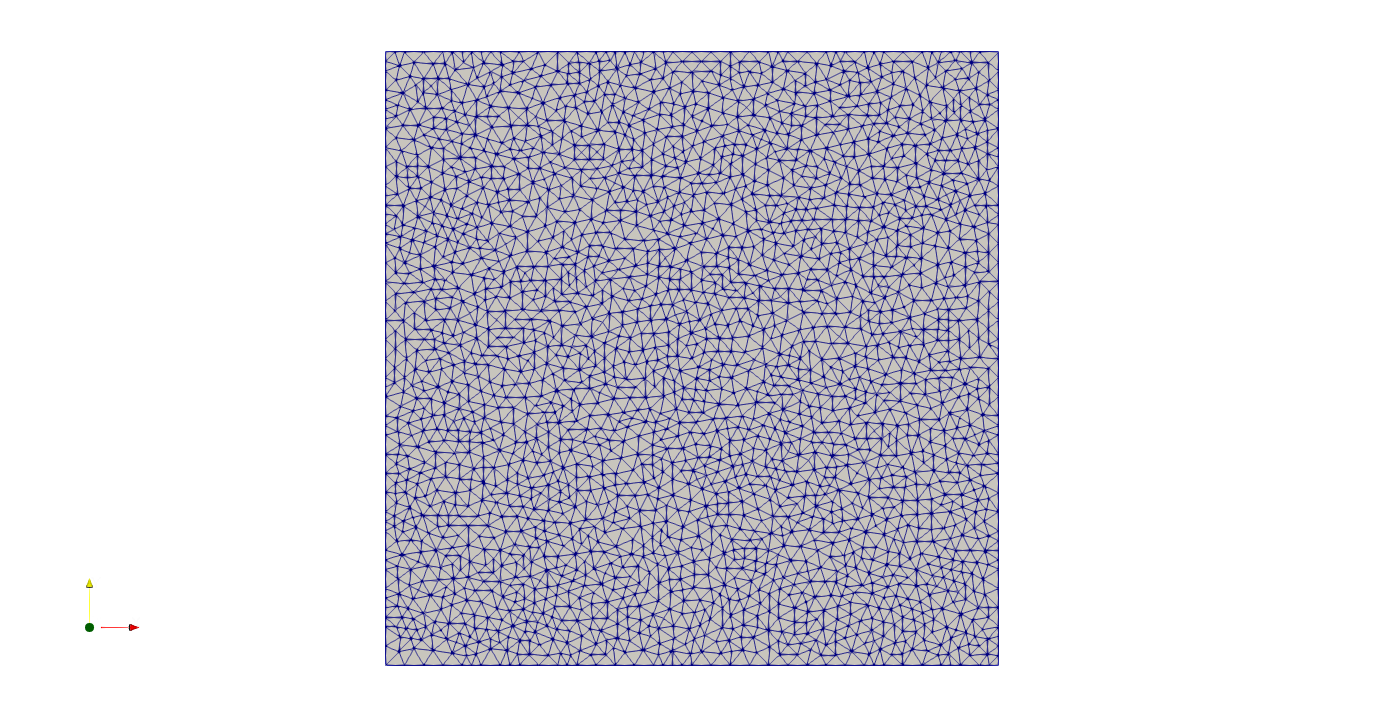
\includegraphics[width=0.4\textwidth]{MeshSquare}}
    \end{figure}
\end{frame}

\begin{frame}
    \frametitle{Startup flow fixed pressure}
    \begin{figure}
        \subfigure{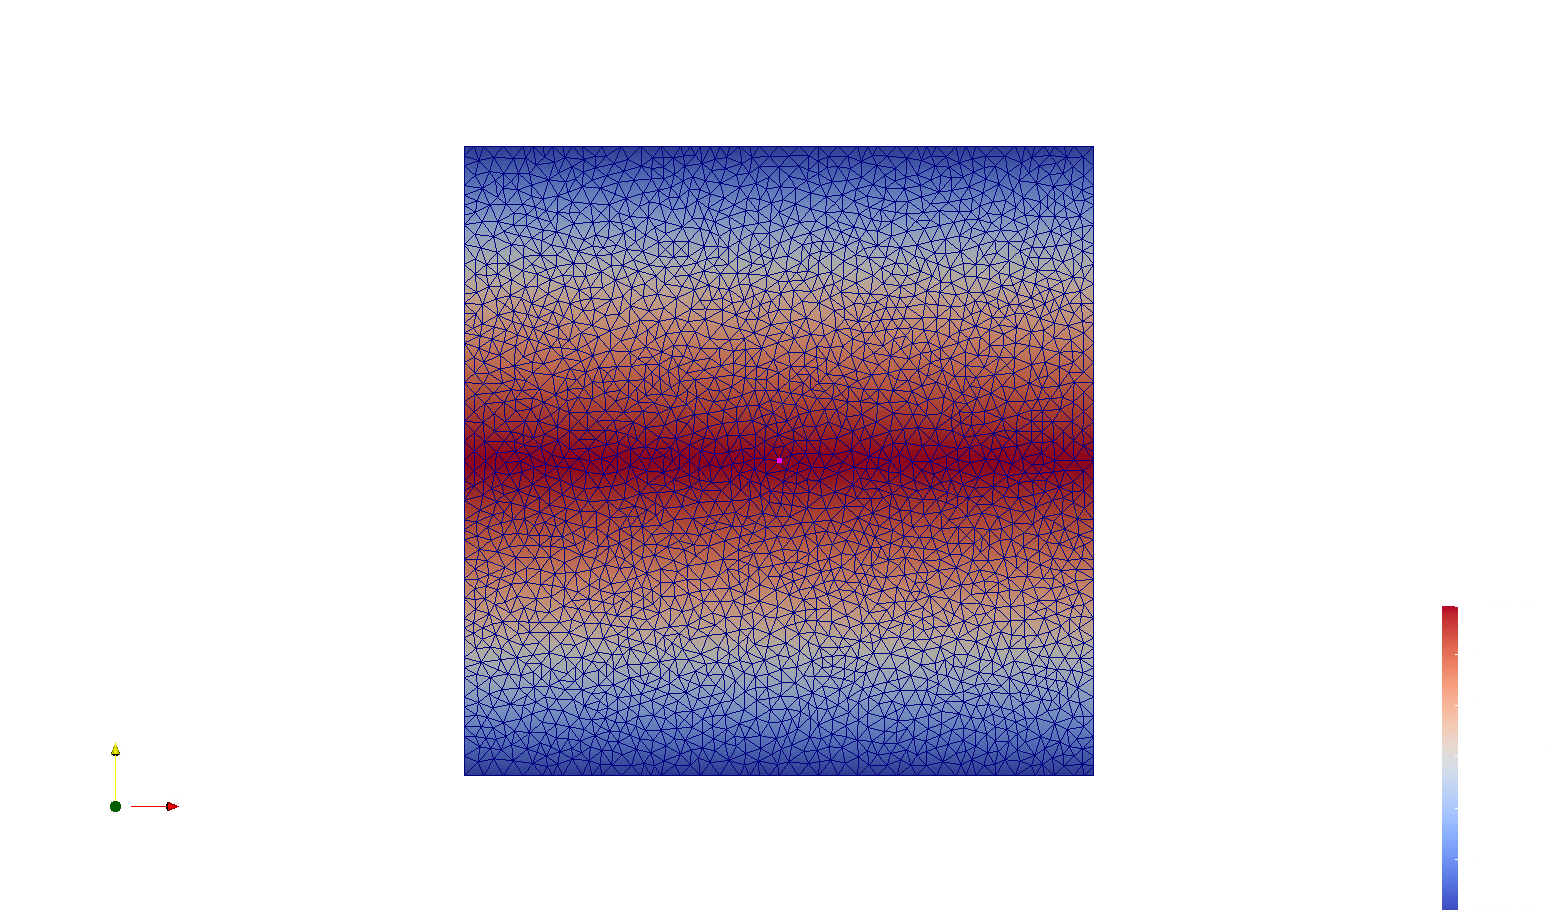
\includegraphics[width=0.4\textwidth]{vel}}
        \subfigure{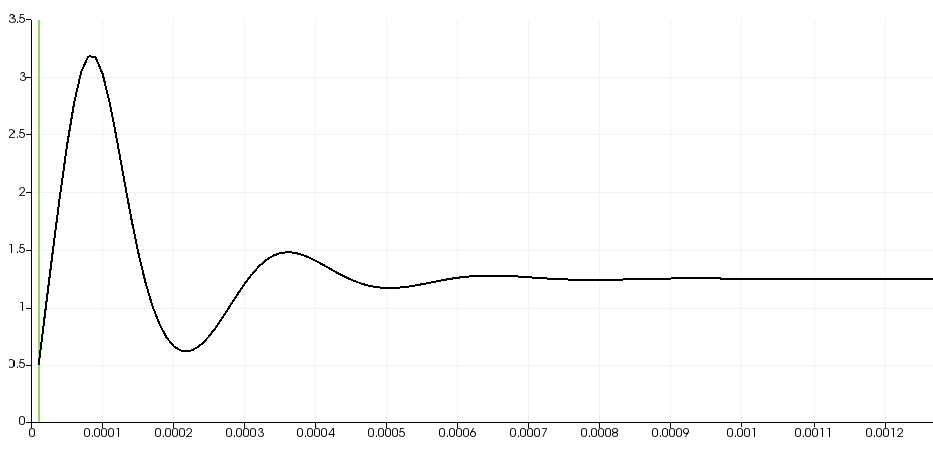
\includegraphics[width=0.5\textwidth]{centerlinevel}}
        \caption{Startup flow Maxwell with $E=1$ and $p=-3$}
    \end{figure}
\end{frame}
\begin{frame}
    \frametitle{Numerical results}
    Convergence in the $L2$-norm was achieved with a timestep width of $0.1$ and an end time of $1$.
    \begin{table}
        \centering
        \begin{tabular}{c|c|c}
            $\approx$ \# Elements per diameter& $\mathrm{L}^2$-error&EOC\\
            \hline
            20 & 0.0797652 & -\\
            40 & 0.0233543 & 1.77207\\
            80 & 0.00615334 & 1.92425\\
            160 & 0.00163421 & 1.91278\\
            320 & 0.000433982 & 1.91288
        \end{tabular}
        \caption{Convergence of the \textsc{Maxwell} model $(\mu_s=0)$}
    \end{table}
\end{frame}
\begin{frame}
    \frametitle{Cross section of an ideal rheometer}
    
\end{frame}
\section{Conclusion and outlook}
\begin{frame}
    \frametitle{Conclusion}
    \begin{itemize}[<+->]
        \item Simulation of a 2D problem 
        \item theoretical existence and uniqueness were proven
        \item results match physical expectations
        \item numerical convergence was obtained in practice
        \item simulation of a flow inside a rheometer cross section
    \end{itemize}
\end{frame}
\begin{frame}
    \frametitle{Outlook}
    Open questions:
    \begin{itemize}[<+->]
        \item For this thesis:
        \begin{itemize}[<+->]
            \item What if the pressure is not constant?
             \item What if the \enquote{Laplace trick} is not possible?
        \end{itemize}
       \item In the long run:
       \begin{itemize}[<+->]
          \item What if the flow is not only limited to one direction? 
          \item How can parallelization speed up the calculation? 
          \item How does one handle a continuous set of relaxation times?
          \item How can one use a simulation to perform parameter estimations?
       \end{itemize}
    \end{itemize}
\end{frame}
\begin{frame}
\huge{Thank you for your attention!}
\end{frame}
\end{document}
